%\twocolumn
\onehalfspacing


%%%%%%%%%%%%%%%%%%%%%%%%%%%%%%%%%%%%%%%%%%%%%%%%%%%%%%%%%%%%%%%%%%%%%%%%%%%%%%%%
\onecolumn
\section{General Information}
Click on very top of the MFD. (on the first line of text, for example) It will pop up the same MFD screen, this clone can be dragged around and will stay on screen.

One can safely push all the buttons MFD has, this will never cause any control issues. This is not the same with other buttons - they might do things that are can hurt the spacecraft.

Click around the buttons on left and right of the MFD before the ascent to change target orbit parameters.

The rocket will initially be put into orbit with a high apogee and a perigee that might be below the planet's surface. This is intentional: the second stage booster that was dropped will burn up in atmosphere shortly.

Some keys can be bound to RCS commands (sim/rcs/xp, ...), but it's also possible to simply push \reg{TRANS INPUT} button to enable the translational input. This will change the joystick from rotational input to translational input.

The big indicator above the \reg{SRB IGNT} button is the orbital counter. It shows how many circles around the Earth have been made.

Remember: burn at apogee changes perigee, burn at perigee changes apogee.


%%%%%%%%%%%%%%%%%%%%%%%%%%%%%%%%%%%%%%%%%%%%%%%%%%%%%%%%%%%%%%%%%%%%%%%%%%%%%%%%
\section{Glossary}

\paragraph{Units of measurement}~
The spacecraft uses metric system of units everywhere. 1 meter is approximately 3 feet, 1 kilometer is approximately 0.5 miles. Water boils at 100 degrees C, and freezes at 0 degrees C.

\paragraph{Orbit}~
A stable trajectory of a very fast moving spacecraft which does not interesect with Earth.

\paragraph{Orbital elements}~
A set of variables which define the orbit, for example apogee and perigee.

\paragraph{Orbital plane}~
An orbit is a trajectory on a single plane. This is called the orbital plane.

\paragraph{Apogee}~
Point at which spacecraft is furthest away from Earth.

\paragraph{Perigee}~
Point at which spacecraft is closest to Earth.

\paragraph{Inclination}~
Rotation of the orbital plane from the Earth equator.

\paragraph{Semimajor axis}~
Defines ellipse that represents the orbit. Is equal to an average between apogee and perigee.

\paragraph{Hohmann transfer}~
An easy and moderately efficient transfer between two orbits. Requires two engine burns.

\paragraph{Semimajor transfer}~
Transfer which only changes either apogee or perigee. Requires just one orbit burn. Two of these make up a Hohmanns transfer.

\paragraph{Heat flux}~
Flow of heat over a unit of area, per unit of time. A measure of how much thermal energy goes through a certain surface.

\paragraph{Velocity vector}~
Mathematical vector, a representation of the direction spacecraft flies towards.

\paragraph{Prograde}~
Oriented along the velocity vector - facing the direction of motion.

\paragraph{Retrograde}~
Oriented against the velocity vector - facing away from the direction of motion.

\paragraph{RCS}~
Reaction control system - a set of small rocket engines used for orienting spacecraft around in space.

\paragraph{OMS}~
Orbital manuevering system - one or more rocket engines used for changing the current orbit.

\paragraph{DAP}~
Digital autopilot - a special computer program which controls spacecraft motion.

\paragraph{MFD}~
Multi-functional display - a computer display which provides various flight information, depending on the current mode (function) selected.

\paragraph{Powered Explicit Guidance}~
A mathematical algorithm which computes trajectory the spacecraft must fly based on its current state, and the state it must have at the end of guidance.

\paragraph{Delta-V}~
Change of the spacecrafts velocity. May be used in context of total delta-V that a spacecraft has - the maximum change of velocity that can be done using its engines.

\paragraph{Burn}~
An orbital manuever which consists of firing an engine into a specific direction to change the spacecraft's velocity.

\paragraph{Re-entry}~
A special manuever which consists of lowering spacecraft into dense atmosphere, and using the friction to reduce its velocity. Generates a massive amount of heat, which is absorbed or reflected by the spacecrafts heat shield.


%%%%%%%%%%%%%%%%%%%%%%%%%%%%%%%%%%%%%%%%%%%%%%%%%%%%%%%%%%%%%%%%%%%%%%%%%%%%%%%%
\onecolumn
\section{Flight Mode Reference}
The on-board software is divided into sections called flight modes. Each flight mode is a distinct portion of the software, and will perform only a certain subset of features. The computer will automatically transfer between these flight modes.

During the on-orbit operations it is possible to change the current mode either by using the event programer, or by using buttons under the MFD.

\begin{center} \begin{tabular}{|c|p{5.0in}|} \hline 
Flight mode & Description \\ \hline 
\reg{00} & Idle \\ \hline 
\reg{10} & Stage 1 ascent (pre-programmed guidance) \\ \hline 
\reg{11} & Stage 1 ascent (active guidance) \\ \hline 
\reg{20} & Stage 2 ascent (early ascent) \\ \hline 
\reg{21} & Escape tower separation \\ \hline 
\reg{22} & Payload fairing separation \\ \hline 
\reg{23} & Stage 2 ascent (late ascent) \\ \hline 
\reg{30} & Stage 3 / On-orbit idle \\ \hline 
\reg{31} & Stage 3 / Kill-Rot autopilot \\ \hline 
\reg{32} & Stage 3 / Att-Pro autopilot \\ \hline 
\reg{33} & Stage 3 / Att-Ret autopilot \\ \hline 
\reg{34} & Stage 3 / Orbital normal + autopilot \\ \hline 
\reg{35} & Stage 3 / Orbital normal - autopilot \\ \hline 
\reg{40} & CM / On-orbit idle \\ \hline 
\reg{41} & CM / Kill-Rot autopilot \\ \hline 
\reg{42} & CM / Att-Pro autopilot \\ \hline 
\reg{43} & CM / Att-Ret autopilot \\ \hline 
\reg{44} & Stage 3 / Orbital normal + autopilot \\ \hline 
\reg{45} & Stage 3 / Orbital normal - autopilot \\ \hline 
\reg{50} & Ballistic reentry stabilization \\ \hline 
\reg{51} & Active atmospheric braking \\ \hline 
\reg{52} & Free flight \\ \hline 
\reg{53} & Parachute descent \\ \hline 
\reg{54} & Braking jets \\ \hline 
\reg{55} & On ground \\ \hline 
\reg{60} & Controlled reentry \\ \hline
\end{tabular} \end{center}


%%%%%%%%%%%%%%%%%%%%%%%%%%%%%%%%%%%%%%%%%%%%%%%%%%%%%%%%%%%%%%%%%%%%%%%%%%%%%%%%
\twocolumn
\section{Cockpit Buttons Reference}
\subsection{Keyboard}
The keyboard is used for programming the on-board event controller.

\subsection{\reg{TRANS INPUT}}
Toggles between translational and rotational control via joystick. The pitch axis will control movement on X axis (forward/backward). The roll axis will control movement on the Y axis (left/right). The yaw axis will control movement on the Z axis (up down).

This mode is used for more precise manuevers when two spacecraft are close together.

\subsection{\reg{LAND JETS}}
Arms the landing jets. They are the rockets which soften touchdown after the capsule landing on Earth.

Landing jets are operated by the flight software, and will fire automatically if armed during landing.

\subsection{\reg{LAZY DAP}}
This button controls fuel consumption and precision of the digital autopilot control. When this button is in pressed state, the autopilot will conserve fuel by making less adjustments to attitude.

\subsection{\reg{PV EXTEND}}
Extends solar panels. Not available in this release.

\begin{figure}[htb]
\centering
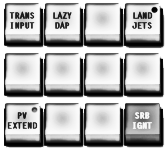
\includegraphics[bb=0 0 5.9cm 5.3cm,scale=0.75]{../graphics/rv550_buttons1.png}
\caption{Buttons on the left panel}
\end{figure}

\subsection{\reg{RCS ON}}
Enables or disables the reaction control system thrusters. These are the thrusters used for orienting ship, changing its attitude.

\subsection{\reg{KILL ROT}}
Changes into flight mode 31. The spacecraft will fire reaction control system jets to stop any residue rotation it might have.

\subsection{\reg{ATT PRO}}
Changes into flight mode 32. The spacecraft will fire reaction control system jets to orient itself along velocity vector.

\subsection{\reg{ATT RET}}
Changes into flight mode 32. The spacecraft will fire reaction control system jets to orient itself against velocity vector.

\subsection{\reg{ORB ENGN}}
Arms the service module engine. This will provide control of the engine (throttle will start it up).

\subsection{\reg{DROP ARM}}
Arms separation of the service module. It is only required for manual separation using the \reg{DROP STAGE} button.

\subsection{\reg{DROP STAGE}}
If \reg{DROP ARM} is pressed, this button will deattach service module from the capsule.

\begin{figure}[htb]
\centering

\includegraphics[bb=0 0 11cm 1.6cm,scale=0.75]{../graphics/rv550_buttons2.png}
\caption{Buttons under the MFD}
\end{figure}


%%%%%%%%%%%%%%%%%%%%%%%%%%%%%%%%%%%%%%%%%%%%%%%%%%%%%%%%%%%%%%%%%%%%%%%%%%%%%%%%
\section{MFD Screens Reference}
\subsection{\reg{FAULT} (Message Log/Fault Display)}
This screen will display all key events, error messages, and notifications that occur during spacecraft operation.

\begin{figure}[htb]
\centering
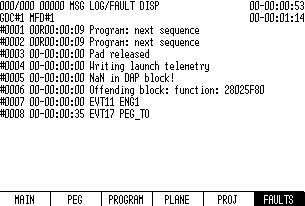
\includegraphics[bb=0 0 9cm 7cm,scale=0.50]{../graphics/rv550_screen3.png}
\end{figure}

\subsection{\reg{SYSTEM} (System Information)}
This MFD screen displays some operating system information.

\begin{figure}[htb]
\centering
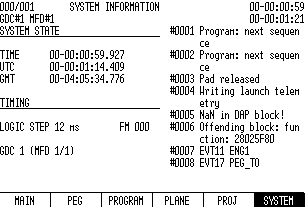
\includegraphics[bb=0 0 9cm 7cm,scale=0.50]{../graphics/rv550_screen4.png}
\end{figure}

\subsection{\reg{SYSDATA} (Internal System Data)}
The Internal System Data screen is used for low-level operating system troubleshooting.

\begin{figure}[htb]
\centering
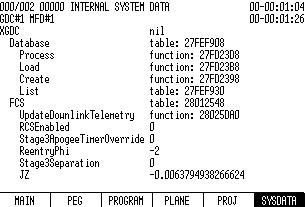
\includegraphics[bb=0 0 9cm 7cm,scale=0.50]{../graphics/rv550_screen5.png}
\end{figure}

\subsection{\reg{FLASHMEM} (Flash Memory)}
Flash memory/filesystem state is displayed on this screen. It lists files and their sizes.

\begin{figure}[htb]
\centering
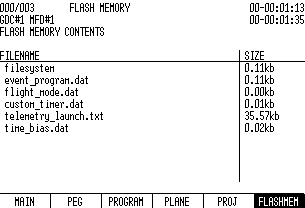
\includegraphics[bb=0 0 9cm 7cm,scale=0.50]{../graphics/rv550_screen6.png}
\end{figure}

\subsection{\reg{PEG} (Powered Explicit Guidance)}
This screen is used for monitoring state of the active guidance during ascent. It displays the following variables:
\begin{itemize}
	\item \reg{Stage}: currently active rocket stage
	\item \reg{Polar angle}: angular distance travelled by the rocket, in radians
	\item \reg{Angular velocity}: angular velocity of the rocket (in Earth-centric inertial coordinates)
	\item \reg{Angular momentum}: total angular momentum of the rocket in the inertial coordinates
	\item \reg{Target radius}, \reg{Target velocity}: target point for the guidance
	\item \reg{Estimated mass}: estimated full mass of the spacecraft stack
	\item \reg{Steering command}: steering command returned by the guidance algorithm
	\item \reg{Target angle}: commanded rocket attitude
	\item \reg{Estimate cutoff}: time till cutoff (end of guidance)
	\item \reg{Delta-V}: velocity that still has to be gained
	\item \reg{Current radius}: current distance from the planet surface
	\item \reg{Radial velocity}: vertical velocity
	\item \reg{Tangent velocity}: groundspeed
\end{itemize}

The additional table lists guidance coefficients for each of the rocket stages.

\begin{figure}[htb]
\centering
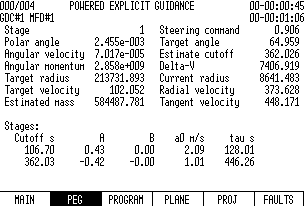
\includegraphics[bb=0 0 9cm 7cm,scale=0.50]{../graphics/rv550_screen2.png}
\end{figure}

%\subsection{\reg{EARTH} (Earth Orbital Views)}

%\subsection{\reg{PLANE} (Orbital Plane View)}

%\subsection{\reg{PROJ} (Projected Orbital View)}

\subsection{\reg{REENTRY} (Reentry Trajectory)}
This screen provides information about computed reentry trajectory. The reentry trajectory is updated continiously.

The following variables are listed:
\begin{itemize}
	\item \reg{Latitude}/\reg{Longitude}: estimated landing coordinates if the de-orbit burn was to be executed just now
	\item \reg{Time to burn}: time remaining to the next reentry opportunity
	\item \reg{Time to best approach}: time remaining to the reentry opportunity that will bring the vessel most close to the target location
	\item \reg{Delta-V}: required change in velocity for the reentry
	\item \reg{Velocity}: current velocity
	\item \reg{Target}: target velocity
	\item \reg{Phi}: angle at which spacecraft will enter the Earth atmosphere
	\item \reg{Lat}/\reg{Lon}: target landing coordinates
\end{itemize}

The small map displays orbital track, and highlights remaining path to target reentry point as a red line. The small red rectangle indicates location of the landing if the burn was to be made just now.


\begin{figure}[htb]
\centering
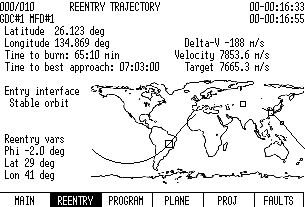
\includegraphics[bb=0 0 9cm 7cm,scale=0.50]{../graphics/rv550_screen7.png}
\end{figure}

\subsection{\reg{OPT RTRAJ} (Optimize Reentry Trajectory)}

This screen is used for optimizing the reentry trajectory for a closer approach to the target landing site. It lists estimates of distance from the landing point to target reentry point.

This table also lists time remaining until that point is reached.

All other displayed variables are the same as on the \reg{REENTRY} screen.

\begin{figure}[htb]
\centering
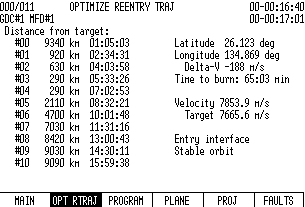
\includegraphics[bb=0 0 9cm 7cm,scale=0.50]{../graphics/rv550_screen8.png}
\end{figure}

\subsection{\reg{MAIN} (Main Flight Display)}
This display provides most important information regarding the spacecraft. It has three distinct sub-screens which are most relevant to the current phase of flight:
\begin{itemize}
	\item Ascent 
	\item On-orbit operations
	\item Re-entry
\end{itemize}

During ascent this screen will display remaining fuel, target command from the guidance software, current altitude and velocity, remaining velocity.

It will also display estimate of time till cutoff, and total elapsed time.

\begin{figure}[htb]
\centering
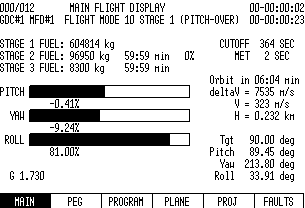
\includegraphics[bb=0 0 9cm 7cm,scale=0.50]{../graphics/rv550_screen1.png}
\end{figure}

During on-orbit operations this screen displays state of all reaction control system thrusters, remaining fuel in RCS and OMS, current velocity vector.

This screen also lists rotation rates and current angles on all three axes, followed by current command (from digital autopilot, and users input).

\reg{R} is the current altitude, while \reg{Rp} and \reg{Ra} are values of perigee and apogee respectively.

This screen also shows a portion of event programmer, displaying next 4 commands to be executed, and time remaining.

\begin{figure}[htb]
\centering
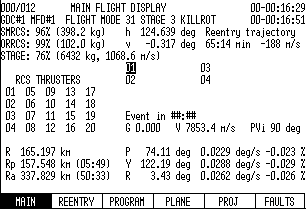
\includegraphics[bb=0 0 9cm 7cm,scale=0.50]{../graphics/rv550_screen0.png}
\end{figure}

\subsection{\reg{ORB BURN} (Orbital Engine Burn)}
This screen lists calculations related to orbital manuevering system burns. It will list remaining fuel in service module and OMS tanks, along with estimate of total delta-V available from these systems.

The table lists amount of time in seconds required to perform a target burn. It lists target change in velocity on the horizontal axis, and target throttle setting on the vertical axis.

\begin{figure}[htb]
\centering
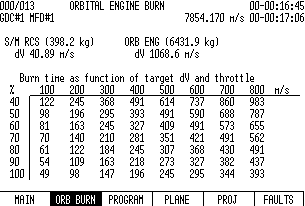
\includegraphics[bb=0 0 9cm 7cm,scale=0.50]{../graphics/rv550_screen9.png}
\end{figure}

\subsection{\reg{HEAT} (Heat Shield Status)}
Heat shield status screen will display temperature values from certain sensors located on the spacecraft bottom.

The large diagram shows estimate of temperature for all sensors and current heat flux at these points.

Heat flux is displayed in kilowatts per one square meter.

\begin{figure}[htb]
\centering
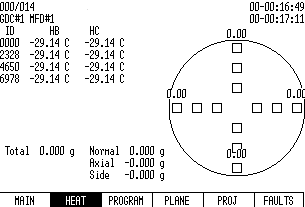
\includegraphics[bb=0 0 9cm 7cm,scale=0.50]{../graphics/rv550_screen10.png}
\end{figure}

%\subsection{\reg{PROGRAM} (Event Programming)}
